\documentclass{article}
\usepackage{graphicx}
\usepackage{amsmath}%
\setcounter{MaxMatrixCols}{30}%
\usepackage{amsfonts}%
\usepackage{amssymb}%
\title{Google Reactor Calibration Model}
\author{Jin Liu}
%\date{February 21, 2017}
\setlength\parindent{0pt}
\begin{document}
\maketitle

This note is to describe the parameters and formula Google IPB Reactor Calibration Model.\\
\\

The proposed equivalent circuit model is described in Figure 1.\\

\begin{figure}
[h]
\begin{center}
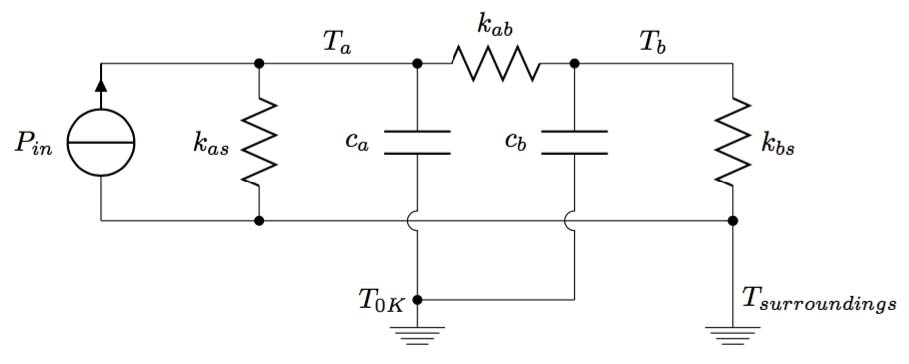
\includegraphics[scale=1]{formula1.jpg} 
\caption{Circuit Model}%
\end{center}
\end{figure} 
The governing equations are:
\begin{equation}
\frac{dT_{a}(t)}{dt}=\frac{P_{in}-k_{as}(T_{a}-T_{s})-k_{ab}(T{a}-T_{b})}{c_{a}}\label{1}%
\end{equation} 

\begin{equation}
\frac{dT_{b}(t)}{dt}=\frac{P_{in}-k_{ab}(T_{a}-T_{s})-k_{bs}(T{b}-T_{s})}{c_{b}}\label{1}%
\end{equation} 

The parameters in the equations are:
\begin{equation}
k_{as}=(k_{as0}+k_{as1}T_{a}+k_{as2}T_{a}^{2})\label{1}%
\end{equation}  
\begin{equation}
k_{ab}=(k_{ab0}+k_{ab1}T_{a}+k_{ab2}T_{a}^{2})
\end{equation}  
\begin{equation}
k_{bs}=(k_{bs0}+k_{bs1}T_{b}+k_{bs2}T_{b}^{2})
\end{equation}  
\begin{equation}
c_{a}=(c_{a0}+c_{a1}T_{a}+c_{a2}T_{a}^{2})
\end{equation}  
\begin{equation}
c_{b}=(c_{b0}+c_{b1}T_{b}+c_{b2}T_{b}^{2})
\end{equation} 

\begin{equation}
P_{in}(t)=(a_{10}+a_{11}T_{a}+a_{12}T_{a}^{2})P_{heaterpower} + (a_{20}+a_{21}T_{a}+a_{22}T_{a}^{2})P_{core-Q}\label{1}%
\end{equation}
in $DC$ $P_{core-Q}$ is $P_{DC}$\\

$T_{a}$ is the core temperature\\
$T_{b}$ is the inner block temperature\\
$T_{s}$ is the outer block temperature\\

\begin{equation}
P_{out}(t)=k_{as}[T_{a}(t)-T_{s}(t)]+k_{bs}[T_{b}(t)-T_{s}(t)]\label{1}%
\end{equation}  

\begin{equation}
P_{stored}(t)=c_{a}\frac{dT_{a}(t)}{dt}+c_{b}\frac{dT_{b}(t)}{dt}\label{1}%
\end{equation}  

The Energy COP defined as
\begin{equation}
COP_{energy}(t)=\frac{\int_{0}^{t}{[P_{out}(t)+P_{stored}(t)]dt}}{\int_{0}^{t}P_{in}(t)dt}\label{1}%
\end{equation}

The Power COP defined as

\begin{equation}
COP_{power}(t)=\frac{{P_{out}(t)+P_{stored}(t)}}{P_{in}(t)}\label{1}%
\end{equation}

The Google Team has done four calibration models, the table 1. lists all the parameters in the calibration models.
\begin{table}[htdp]
\centering
\caption{Parameters in Google Model}

\begin{tabular}{|c|c|c|c|c|c|c|}
\hline
Paras & ipb1-30-he & ipb1-30-h2 & sri-ipb2-27-h2 & sri-ipb2-33-he & sri-ipb2-33-h2 & ipb1-40-he\\ \hline
ca0	&	10.58	&	52.91	&	17.19	&	20.59	&	18.381	&	22.708	\\	\hline
ca1	&	4.30E-01	&	2.20E-01	&	-6.77E-01	&	8.57E-02	&	1.52E-01	&	1.89E-02	\\	\hline
ca2	&	-9.39E-04	&	-2.66E-04	&	8.59E-03	&	1.22E-05	&	-3.49E-05	&	1.71E-05	\\	\hline
cb0	&	601.10	&	579.90	&	883.48	&	675.09	&	666.22	&	777.96	\\	\hline
cb1	&	0.46692	&	0.38258	&	-2.75100	&	0.12088	&	0.11378	&	-0.18899	\\	\hline
cb2	&	0	&	0	&	0	&	0	&	0	&	0	\\	\hline
kas0	&	2.92E-02	&	2.66E-02	&	5.15E-05	&	1.72E-03	&	5.14E-03	&	-8.13E-03	\\	\hline
kas1	&	-5.31E-05	&	-2.70E-05	&	2.35E-04	&	4.62E-05	&	3.99E-05	&	2.49E-05	\\	\hline
kas2	&	0	&	0	&	0	&	0	&	0	&	0	\\	\hline
kab0	&	0.65350	&	0.61924	&	0.82998	&	0.56864	&	0.54634	&	0.78189	\\	\hline
kab1	&	-4.87E-04	&	7.96E-04	&	-2.40E-03	&	8.19E-04	&	7.95E-04	&	9.41E-04	\\	\hline
kab2	&	3.66E-06	&	1.00E-06	&	1.75E-06	&	-4.38E-07	&	-2.63E-07	&	-3.23E-07	\\	\hline
kbs0	&	0.03301	&	0.03681	&	0.07530	&	0.06369	&	0.06328	&	0.06637	\\	\hline
kbs1	&	1.57E-04	&	1.21E-04	&	-2.66E-04	&	5.80E-05	&	4.04E-05	&	7.85E-05	\\	\hline
kbs2	&	6.54E-08	&	7.53E-08	&	2.74E-07	&	2.50E-08	&	7.29E-08	&	4.11E-08	\\	\hline
a10	&	1	&	1	&	1	&	1	&	1	&	1	\\	\hline
a11	&	0	&	0	&	0	&	0	&	0	&	0	\\	\hline
a12	&	0	&	0	&	0	&	0	&	0	&	0	\\	\hline
a20	&	0.367580	&	0.359820	&	0.425000	&	0.050546	&	0.28613	&	0.049953	\\	\hline
a21	&	1.01E-03	&	6.65E-04	&	-9.20E-04	&	3.12E-03	&	1.46E-03	&	3.92E-03	\\	\hline
a22	&	-9.89E-07	&	-9.54E-08	&	4.49E-06	&	-4.38E-06	&	-1.54E-06	&	-5.81E-06	\\	\hline




\end{tabular}
\end{table}

\end{document}
